\documentclass[12pt,parskip]{komatufte}
\usepackage[subpreambles=false]{standalone}

%%%%%%%%%%%%%%%%%%%%%%%%%%%
% Silence warning messages
\usepackage{silence}
\WarningsOff[scrlayer-notecolumn]
\WarningsOff[biblatex]

%%%%%%%%%%%%%%%%%%%%
% Commenting

%\usepackage[author=Lyndon]{pdfcomment}
%\newcommand{\pdfcomment}[1]{} %ignore all comments

%\usepackage{todonotes}
%\newcommand{\pdfcomment}{\todo}


%%%%%%%%%%%%%%%%%%%%
% Tables
\usepackage{booktabs}

%%%%%%%%%%%%%%%%%%%
% Fonts
\usepackage{tgadventor} %sans
\usepackage{tgpagella}  %serif
\usepackage{inconsolata} %mono
\usepackage[T1]{fontenc}

\usepackage{microtype}
\usepackage[all]{nowidow}
%%%%%%%%%%%%%%%%%%%%%%%
% Styling
\setcounter{secnumdepth}{4}
\setcounter{tocdepth}{2}

\usepackage{placeins}



%%%%%%%%%%%%%%%%%%%
% Math
\usepackage{amsmath, amssymb, stmaryrd, mathtools}
\DeclareMathOperator*{\argmin}{argmin}
\DeclareMathOperator*{\argmax}{argmax}

\usepackage{xparse,xstring,etoolbox}
% crossref this against notation section
\newcommand{\vv}[1]{\tilde{#1}} % vector
\newcommand{\seq}[1]{\mathcal{#1}} % sequence
\newcommand{\set}[1]{\mathbb{#1}} % set

%%%%%%%%%
% Indexing/sequence indexing
\newcommand{\seqind}[2]{#1^{#2}} % seqence index
\newcommand{\ind}[2]{#1_{#2}} % indexed
\newcommand{\disamb}[2]{#1^{\mathrm{#2}}} %disambiguated

%% Smart indexing and naming
\newcommand{\ifupper}[3]{
    \normalexpandarg
	\exploregroups
	\StrCount{ABCDEFGHIJKLMNOPQRSTUVWXYZ}{#1}[\uppercount]
	\ifnumgreater{\uppercount}{0}{#2}{#3}
}

%smart index
\DeclareDocumentCommand{\ii}{u{_} m}{
	\ifupper{#1}%
	{% just a single uppercase character, i.e. a matrix
		  %make sure the index is the right length
		\StrCount{#2}{,}[\indcount]
		\ifnumgreater{\indcount}{0}
		{ % Got multiple indexes so all good
		 	\ind{#1}{#2}
		}
		{ % Only 1 index so grab the column
		 	\ind{#1}{{:,#2}}
		}
	}%
	{% Not just a single upper case character
		\ind{#1}{#2}
	}
}

\DeclareDocumentCommand{\nn}{u{_} m}{
	\seqind{#1}{#2}
}

\DeclareDocumentCommand{\dd}{u{_} m}{
	\disamb{#1}{#2}
}

% Index of a vector
\DeclareDocumentCommand{\iv}{u{_} m}{\ii{\vv #1}_{#2}}
\DeclareDocumentCommand{\dv}{u{_} m}{\dd{\vv #1}_{#2}}
\DeclareDocumentCommand{\nv}{u{_} m}{\nn{\vv #1}_{#2}}

%exp
\let\oldexp\exp
\renewcommand{\exp}[1]{\oldexp \left( #1 \right)}
\newcommand{\exptwo}[1]{\oldexp_2 \left( #1 \right)}

\newcommand{\softmax}{\mathrm{smax}}

\DeclareMathOperator*{\expectedop}{\mathbb{E}}
\DeclareDocumentCommand{\expected}{u{_} m}{
	\expectedop\limits_{\mathrlap{#2}}
}

%%%%%%%%%%%%%%%%
%Graphics
\usepackage{tikz}
\usetikzlibrary{positioning, fit,  shapes.geometric}
\usepackage{ifthen}
\usepackage{etoolbox}

\tikzset{
	backgroundcolor/.style ={fill=white},
	every node/.append style={
		minimum height=7mm,
	},
	labe/.append style={
		%Blue,
		align = center,
		backgroundcolor,
		fill opacity=0.6,
		text opacity=1,
		font={\footnotesize\itshape}	
	},
	layer/.append style={
		draw,
		align = center,
		minimum height=7mm,
	},
	tight/.append style={
		inner sep=0.2mm,
	},
	lookupbox/.append style={
		draw=none,
		append after command={
		       	[shorten <= -0.5\pgflinewidth]
		       	([shift={(-1.5\pgflinewidth,-0.5\pgflinewidth)}]\tikzlastnode.north east)
		       	edge([shift={( 0.5\pgflinewidth,-0.5\pgflinewidth)}]\tikzlastnode.north west) 
		       	([shift={( 0.5\pgflinewidth,-0.5\pgflinewidth)}]\tikzlastnode.north west)
		       	edge([shift={( 0.5\pgflinewidth,-1.5\pgflinewidth)}]\tikzlastnode.south west)            
		       	([shift={( -1.5\pgflinewidth,+0.5\pgflinewidth)}]\tikzlastnode.south east)
		       	edge([shift={(-1.5\pgflinewidth,-0.5\pgflinewidth)}]\tikzlastnode.north east)
		},
		inner sep=0.7mm,
		outer sep=0mm,
		minimum width=25mm
	}
}

\usepackage{pgfplots}
\pgfplotsset{compat=1.14}
\pgfplotsset{sideplot/.append style={
		width=\notescolwidth,
		domain=-10:10,
		samples=101,
		smooth,
		enlarge y limits={abs=2},
		axis lines=middle,
		xlabel  = $z$,
		ylabel  = $y$,
	},
	equ/.append style={
		color=blue,
		thick,
		mark=none
	}
}

% Function  For a plot 
% it  needs to be declared in preamble because of how \makenote* interacts with multiple files
\def\errorsurface(#1,#2){(0.5*#1 + 0.7*#2 + sin(deg(1.5*#1 + #2^2)))^2}


\usepackage{graphicx}
\graphicspath{{./figs/}, {./}, {./figs/chaptersentencerrepr/}, {./figs/chapterintromachinelearning/}, {./figs/chapterwordrepr/}}
\usepackage{adjustbox}


%%%%%%%%%%%%%%%%%%%
% Refs
\usepackage{cleveref}

\addbibresource{master.bib}

%%%%%%%%%%%%%%%%%%%%
% Formatting

% for examples from natural language space.
\newcommand{\natlang}[1]{\ifmmode \text{``\texttt{#1}''} \else {``\texttt{#1}''}\fi}
% \ifmmode ``trick'' from https://tex.stackexchange.com/a/15194/5834

%%%%%%%%%%%%%%%%%%%%%


\begin{document}
	
\setchapterpreamble{%
	\dictum[The output of an RNN trained by Andrej Karpathy (2015), trained on an article on the use of RNNs for generating text (it works poorly due to the very low amount of training data). 	\url{http://karpathy.github.io/2015/05/21/rnn-effectiveness/}]{I've the RNN with and works, but the computed with program of the 
		RNN with and the computed of the RNN with with and the code}

}
\chapter{Recurrent neural networks for sequential processing}\label{sec:rnn}
\begin{abstract}
	This chapter continues on from the general introduction to machine learning, with a focus on recurrent networks.
	Recurrent neural networks are the most neural network approach for  working with sequences of dynamic size.
	As with the prior chapter, readers familiar with RNNs can reasonably skip this also;
	it does not pertain specifically to NLP.
	However, as NLP tasks are almost always sequential in nature, RNNs are a very important technique
\end{abstract}

\section{Recurrent Neural Networks}
A key limitation of a neural network is that the number of inputs and outputs must be known at training time and must always be the same for all cases.
This is not true for natural language: If a problem involves processing a sentence, then each input will be made up a varying number of words. Similarly for output, in a text generation case.

Recurrent neural networks (RNN) overcome this by allowing the network to have state that persists over time.
Inputs of any size can be handled one constant sized part of the input (e.g. one word) at a time, using the state to remember past inputs.


A RNN is effectively a chain of feed-forward neural networks,
each one being identical in terms of their weight and bias parameters.
Whiled identical in terms of parameters, they each acting at a different time-step.


\begin{figure}
	\caption{The unrolled structure of an RNN for us in Encoding, Decoding and Encoding-Decoding (sequence-to-sequence) problems. RU is the recurrent unit -- the neural network which reoccurs at each time step.}
	
	\label{fig-rnns}
	
	\resizebox{\textwidth}{!}{\documentclass[landscape]{article}
\usepackage[a3paper]{geometry}

\usepackage{tikz}
\usetikzlibrary{positioning, fit,  shapes.geometric}
\usepackage{ifthen}
\usepackage{etoolbox}

\tikzset{
	backgroundcolor/.style ={fill=white},
	every node/.append style={
		minimum height=7mm,
	},
	labe/.append style={
		%Blue,
		align = center,
		backgroundcolor,
		fill opacity=0.6,
		text opacity=1,
		font={\footnotesize\itshape}	
	},
	layer/.append style={
		draw,
		align = center,
		minimum height=7mm,
	},
	tight/.append style={
		inner sep=0.2mm,
	},
	lookupbox/.append style={
		draw=none,
		append after command={
		       	[shorten <= -0.5\pgflinewidth]
		       	([shift={(-1.5\pgflinewidth,-0.5\pgflinewidth)}]\tikzlastnode.north east)
		       	edge([shift={( 0.5\pgflinewidth,-0.5\pgflinewidth)}]\tikzlastnode.north west) 
		       	([shift={( 0.5\pgflinewidth,-0.5\pgflinewidth)}]\tikzlastnode.north west)
		       	edge([shift={( 0.5\pgflinewidth,-1.5\pgflinewidth)}]\tikzlastnode.south west)            
		       	([shift={( -1.5\pgflinewidth,+0.5\pgflinewidth)}]\tikzlastnode.south east)
		       	edge([shift={(-1.5\pgflinewidth,-0.5\pgflinewidth)}]\tikzlastnode.north east)
		},
		inner sep=0.7mm,
		outer sep=0mm,
		minimum width=25mm
	}
}
\usepackage{amsmath, amssymb, stmaryrd, mathtools}
\DeclareMathOperator*{\argmin}{argmin}
\DeclareMathOperator*{\argmax}{argmax}

\usepackage{xparse,xstring,etoolbox}
% crossref this against notation section
\newcommand{\vv}[1]{\tilde{#1}} % vector
\newcommand{\seq}[1]{\mathcal{#1}} % sequence
\newcommand{\set}[1]{\mathbb{#1}} % set

%%%%%%%%%
% Indexing/sequence indexing
\newcommand{\seqind}[2]{#1^{#2}} % seqence index
\newcommand{\ind}[2]{#1_{#2}} % indexed
\newcommand{\disamb}[2]{#1^{\mathrm{#2}}} %disambiguated

%% Smart indexing and naming
\newcommand{\ifupper}[3]{
    \normalexpandarg
	\exploregroups
	\StrCount{ABCDEFGHIJKLMNOPQRSTUVWXYZ}{#1}[\uppercount]
	\ifnumgreater{\uppercount}{0}{#2}{#3}
}

%smart index
\DeclareDocumentCommand{\ii}{u{_} m}{
	\ifupper{#1}%
	{% just a single uppercase character, i.e. a matrix
		  %make sure the index is the right length
		\StrCount{#2}{,}[\indcount]
		\ifnumgreater{\indcount}{0}
		{ % Got multiple indexes so all good
		 	\ind{#1}{#2}
		}
		{ % Only 1 index so grab the column
		 	\ind{#1}{{:,#2}}
		}
	}%
	{% Not just a single upper case character
		\ind{#1}{#2}
	}
}

\DeclareDocumentCommand{\nn}{u{_} m}{
	\seqind{#1}{#2}
}

\DeclareDocumentCommand{\dd}{u{_} m}{
	\disamb{#1}{#2}
}

% Index of a vector
\DeclareDocumentCommand{\iv}{u{_} m}{\ii{\vv #1}_{#2}}
\DeclareDocumentCommand{\dv}{u{_} m}{\dd{\vv #1}_{#2}}
\DeclareDocumentCommand{\nv}{u{_} m}{\nn{\vv #1}_{#2}}

%exp
\let\oldexp\exp
\renewcommand{\exp}[1]{\oldexp \left( #1 \right)}
\newcommand{\exptwo}[1]{\oldexp_2 \left( #1 \right)}

\newcommand{\softmax}{\mathrm{smax}}

\DeclareMathOperator*{\expectedop}{\mathbb{E}}
\DeclareDocumentCommand{\expected}{u{_} m}{
	\expectedop\limits_{\mathrlap{#2}}
}

\begin{document}

\numdef{\N}{8}
\numdef{\labelwidth}{5.5cm}
%%%%%%%%%%%%%%%%%%%%%%%%%
% Encoder

\begin{tikzpicture}[]

\begin{scope}
	\node(lblEncoder)[text width= \labelwidth] {\textbf{RNN Encoder:}\\%
	Variable $n$ inputs: $\nv x_t$\\%
	1 output: $\hat{y}$ \\%
	};
	
	\coordinate (L0) at (lblEncoder.east);
	
	\foreach \I[count=\j from 0] in {1,...,\N}{
		\ifnumequal{\I}{\N - 1}{%
			\node(L\I)[dashed, layer, right = of L\j] {...};
			\node(w\I)[below = of L\I]{...};
		}%
		{	
			\node(L\I)[layer, right = of L\j] {RU};
			\node(w\I)[below = of L\I]{\ifnumequal{\I}{\N}{$\nv x_n$}{$\nv x_\I$}};
			\draw[->](w\I) -- (L\I);
		}
	}
	\foreach \I[count=\j from 1] in {2,...,\N} {
		\draw[->] (L\j) edge node[labe]{state} (L\I);
	}
	
	\node(out) [above = of L\N]{$\hat{y}$};
	\draw[->] (L\N) -- (out);
\end{scope}

%%%%%%%%%%%%%%%%
% Decoder
\begin{scope}[yshift=-5cm] 
\node(lbl)[text width= \labelwidth] {\textbf{RNN Decoder:}\\%
1 input: $x$\\%
variable $m$ outputs: $\n \hat{y}_t$ \\%
with prompts: $\nv r_t$ (often $\nv y_{t-1}$)
};

\coordinate (L0) at (lbl.east);
\coordinate (L1c)[right = of L0];
\node(x)[below right = 4 of L1c]{$x$};

\foreach \I[count=\j from 0] in {1,...,\N}{
	\ifnumequal{\I}{\N - 1}{%
		\node(L\I)[dashed, layer, right = of L\j] {...};
		\node(w\I)[above = of L\I]{...};
		\node(y\I)[below = of L\I]{...};
	}%
	{	
		\node(L\I)[layer, right = of L\j] {RU};
		\node(v\I)[above = of L\I]{\ifnumequal{\I}{\N}{$\n \hat{y}_m$}{$\n \hat{y}_\I$}};
		\node(w\I)[below = of L\I]{$[\nv r_\I; \v x]$};
		\draw[->](w\I) -- (L\I);
		\draw[->](L\I) -- (v\I);
		\draw[->](x) to[bend right = 5] (w\I.300);
	}
}
\foreach \I[count=\j from 1] in {2,...,\N} {
	\draw[->] (L\j) edge node[labe]{state} (L\I);
}

\end{scope}
%
%%%%%%%%%%%%%%%%%%
% Encoder Decoder
%
\begin{scope}[yshift=-14cm]
\node(lbl)[text width= \labelwidth] {\textbf{RNN Encoder-Decoder:}\\%
Variable $n$ inputs: $\nv x_t$\\%
Variable $m$ outputs $\n \hat{y}_t$\\%
Prompts: $\nv r_t$ (often $y_{t-1}$)
};

\coordinate (L0) at (lbl.east);
\numdef{\NN}{4}
\foreach \I[count=\j from 0] in {1,...,\NN}{
	\ifnumequal{\I}{\NN - 1}{%
		\node(L\I)[dashed, layer, right = of L\j] {...};
		\node(w\I)[below = of L\I]{...};
	}%
	{
		\node(L\I)[layer, right = of L\j] {$\mathrm{RU_E}$};
		\node(w\I)[below = of L\I]{\ifnumequal{\I}{\NN}{$\nv x_n$}{$\nv x_\I$}};
		\draw[->] (w\I) -- (L\I);
	}
}
\foreach \I[count=\j from 1] in {2,...,\NN} {
	\draw[->] (L\j) edge node[labe] {state} (L\I);
}




\coordinate[above = 3 of L\NN] (Lp\NN);
\numdef{\NP}{\N - 1}
\foreach \j in {\NN,...,\NP}{
	\numdef{\I}{\j+1}
	\numdef{\y}{\I - \NN}
	\ifnumequal{\I}{\N-1}{%
		\node(Lp\I)[dashed, layer, right = of Lp\j] {...};
		\node(w\I)[below = of Lp\I]{...};
		\node(y\I)[above = of Lp\I]{...};
	}%
	{
		\node(Lp\I)[layer, right = of Lp\j] {$\mathrm{RU_D}$};
		\ifnumequal{\I}{\N}{
			\node(w\I)[below = of Lp\I]{$[\v z; \nv r_m]$};
			\node(y\I)[above = of Lp\I]{$\n \hat{y}_m$};
		}
		{
			\node(w\I)[below = of Lp\I]{$[\v z; \nv r_\y]$};
			\node(y\I)[above = of Lp\I]{$\n \hat{y}_\y$};
		}

		\draw[->] (w\I) -- (Lp\I);
		\draw[->] (Lp\I) -- (y\I);
		\path[->] (L\NN.north) edge node[labe]{$\v z$} (w\I.south west);
	}
}


\numdef{\NNp1}{\NN + 1}
\foreach \I in {\NNp1,...,\NP} {
	\numdef{\j}{\I+1}
	\draw[->] (Lp\I) edge node[labe] {state} (Lp\j);
}
 

\end{scope}


\end{tikzpicture}




\end{document}}
\end{figure}

\aside[Time-Step]{ RNNs are normally described in terms of a time-step.
	This is the advancement of the system such that the previous output state, is now the input old-state.
	This doesn't have to be literal time -- indeed it can not be, as it is discrete.
	In most NLP applications it is time analogous: words in the order they are said.
	In other NLP applications it might actually be words in the reverse order to that in which they are normally said.
	In other machine learning applications it may not correspond to time at all.
	For example, using a rotating distance sensor (e.g radar) each time-step corresponds to a different angle of the antenna.
}

At each time-step the same network is used, with different inputs.
For purposes of looking at this in the big picture we will first consider each network a black-box recurrent unit (RU).


The recurrent unit takes at each time-step, an input for that time-step, some representation its of state for the RU at the previous timestep; and it produces an output for this time-step, and its state representation for the next time-step.
A diagram of this is shown in \Cref{fig-ru}.
It is worth distinguishing the unit output is not the same as the overall network output, it is just the output of this sub-network at this time-step.
Every-time step can be considered as having two effective inputs (previous state, and actual input at this time-step) and two effective outputs (next state and actual output at this time step).

Not all of these inputs and outputs are actually used at all time steps meaningfully.
The initial state for the first time step is normally set to some zero vector,
and the final state at end of the sequence of normally discarded.
Similar things are done for inputs and outputs depending on the type of problem (decoder/encoder) that the RNN is being used for.

\section{General RNN structures}
In general most interested uses of recurrent networks can be considers belongs to one of 4 general types of structure.
Matched-sequence, encoder, decoder, and encoder-decoder.
These common structures are shown in \Cref{fig-rnns}.
The motivation for using an RNN is if the size of the input and/or the size of the output is not consistent across all cases.

If the input size and the output size is always the same then one can use an matched-sequence RNN structure.
This is the most basic RNN structure.
At each time-step, there is an input, and a target output.
An example of this in natural language processing is part of speech (POS) tagging.
Every word is to be labelled as a noun, a verb, an adjective etc.
This does require memory as the other words around the word being classified influence the correct POS.
Since the same word can occupy a different part of speech depending on the usage.
For example \natlang{record} is both a noun and a verb (it is in-fact almost ubiquitous that all verbs have a noun form).
This particular example is a good use for a Bidirectional RNN (\Cref{sec:bidirection-rnns}), as both the previous and following words are useful for determining the POS.
A key limitation of the matched-seqence structure is that the input and output size must be the same.
Often though one would like to process an input that could be any size, but produce just a fixed size output.



For example if one is trying to learn a mapping from a textual color names into a probability distribution in color-space \pcite{2017arXiv170909360W}, then different descriptions have different numbers of words.
One input might be \natlang{very light green}, while another just \natlang{orange}.
At each time-step one input is provided -- being one of the words in the (potentially multi-word) color name.
Another example use is sentiment analysis, predicting the sentiment being expressed by a sentence as positive or negative.
All the outputs at all time-steps except the last can be ignored.
The output of the final time-step can be connected to connected to a further network with a final output layer giving the overall output.
This situation with a variable number of inputs but a fixed size of output is described as an encoder network.

\aside[Pseudo-tokens]{
	Pseudo-tokens such as \natlang{<EOS>} (end of string),
	\natlang{<START>} (start of string), and similar are common in RNN tasks.
	As mentioned, outputting \natlang{<EOS>} is required to known when the decode is done outputting.
	\natlang{<START>} can be useful to model things that occur near the start of input; and as an initial prompt.
	In some tasks other non-word tokens might be inserted also.
	Such as in transcription of recorded speech, a \natlang{<PAUSE>} token might be included.
	Pragmatically, as long a the symbols used to represent these never occur amongst the true word tokens, these can be treated just like regular words by the system.
}


The reverse is a decoder network.
This means a fixed sized input mapping to a variably sized output.
If the system is attempting to learn from a point in color space to the name of that color \pcite{2016arXiv160603821M}.
For example: \texttt{(144,238,144)} \natlang{very light green} (3 outputs); but \texttt{(255,165,0)} might map to just \natlang{orange} (one output).
In this decoder type network, there is one true input, at the first time-step, and the output from every time-step is used.
Each output can be connected to a softmax layer giving probability for possible words.
Some inputs at each time-step after the first in such a network inputs must also be provided for the decoding.
We call this input a prompt, as it is not providing new information to the network, merely driving it to produce the next output.
It is common to include an end of string marker token (often literally `\natlang{<EOS>}`),
so as to know when to stop prompting for additional outputs.


The encoder-decoder RNN is the generalise structure for sequence to sequence learning \pcite{cho-EtAl:2014:EMNLP2014}.
While the matched-sequence RNN take a sequence as an input and produces a sequence as an output those sequences must be the same size.
In an application such as machine translation, or question answering, or automatic captioning, sequential input and output is required, but the sequences have different lengths.
A sentence in one language will not normally translate to a sentence with the exact same number of word in another.
The solution to this is the encoder-decoder RNN.
In this structure an encoder RNN is used to take the input, its final output is then connected as the input to so a separate decoder RNN.
Thus separating the input processing from the output generation.


\subsection{Prompts in decoder RNNs}

\aside[Terminology: Prompt]{
	The word prompt is out own terminology here.
	We are not aware of a consistent term used in literature for the input at each time step to a decoder RNN.
	Dummy input would also work,
	although as discussed the chose of prompt can allow useful information to be added.
	Simplifying the learning problem.
}

Prompts are required for decoders as the network must has some input to cause it to give an output.
In theory this could be a constant: all inputs and all outputs for those inputs, can be learned and remembered by the networks memory (encoded in its state).
In practice is very common to include part of the output of the previous step as part of the prompt.
When generating a sequence of words for example, one can use the previous word.
At training time this can be the targeted previous output.
At test time (and in real deployment) this is normally the most-likely predicted output.
This effectively gives direct bigram state information to the model,
allowing the memory to focus on higher level tasks.
It also allows allows the outputs to be explored, for example by providing the second most-likely word as the first prompt a different sequence can be generated.

It is also common to include in prompts the original input to the decoder.
For example in a caption generator, including the a vector representation of the image (for example an Inception Image Embedding); in the color decoder example this would be including the original color representation.
In general the prompt can be used to add information to the network ensuring that each time step can do as well as possible, even if the state does not capture all the information desired.
Ensuring the state is able to capture all information is part of designing the internals of the RU.


\section{Inside the Recurrent Unit}
\begin{figure}
	\caption{A recurrent unit with its 2 inputs and 2 outputs. Not shown are the internal functioning which may be a complex (or simple) neural network of its own.}	
	
	\label{fig-ru}
	
	\documentclass{standalone}

\usepackage{tikz}
\usetikzlibrary{positioning, fit,  shapes.geometric}
\usepackage{ifthen}
\usepackage{etoolbox}

\tikzset{
	backgroundcolor/.style ={fill=white},
	every node/.append style={
		minimum height=7mm,
	},
	labe/.append style={
		%Blue,
		align = center,
		backgroundcolor,
		fill opacity=0.6,
		text opacity=1,
		font={\footnotesize\itshape}	
	},
	layer/.append style={
		draw,
		align = center,
		minimum height=7mm,
	},
	tight/.append style={
		inner sep=0.2mm,
	},
	lookupbox/.append style={
		draw=none,
		append after command={
		       	[shorten <= -0.5\pgflinewidth]
		       	([shift={(-1.5\pgflinewidth,-0.5\pgflinewidth)}]\tikzlastnode.north east)
		       	edge([shift={( 0.5\pgflinewidth,-0.5\pgflinewidth)}]\tikzlastnode.north west) 
		       	([shift={( 0.5\pgflinewidth,-0.5\pgflinewidth)}]\tikzlastnode.north west)
		       	edge([shift={( 0.5\pgflinewidth,-1.5\pgflinewidth)}]\tikzlastnode.south west)            
		       	([shift={( -1.5\pgflinewidth,+0.5\pgflinewidth)}]\tikzlastnode.south east)
		       	edge([shift={(-1.5\pgflinewidth,-0.5\pgflinewidth)}]\tikzlastnode.north east)
		},
		inner sep=0.7mm,
		outer sep=0mm,
		minimum width=25mm
	}
}

\begin{document}

\numdef{\n}{8}
%%%%%%%%%%%%%%%%%%%%%%%%%
% Encoder

\begin{tikzpicture}[]

\node(ru)[layer]{RU};

\node(stm)[left = of ru]{old state};
\draw[->] (stm) edge node[labe] {$s_{t-1}$} (ru);

\node(stp)[right = of ru]{new state};
\draw[->] (ru) edge node[labe] {$s_{t}$} (stp);


\node(out)[above = of ru]{output};
\draw[->] (ru) edge node[labe] {$\hat{y}_t$} (out);


\node(in)[below = of ru]{input};
\draw[->] (in) edge node[labe] {$x_t$} (ru);


\end{tikzpicture}

\end{document}
\end{figure}

\aside[Output/Input layers]{
	Extra feedfordward layers are often applied between the overall networks input and output and the RU's input an output.
	The extra layers could be considered as considered part of the RU, as they occur at each time-step (even if not used).
	Alternatively they can be considered as  something that surrounds the RU, only at certain time-steps.
	This depends on depending on point of view.
	For out purposes we will consider the core of the RU in isolation.
}

In this section we discuss the various different types of recurrent unit.
This is the different between Elman networks, GRU networks and LSTM networks.
As discussed every recurrent unit from the outside has the previous state, the next state, the unit input and the unit output.
What differs is how they are connected and what controls the information with in them.
Every recurrent unit is itself a neural network.

In many types of RU (e.g. GRU, Basic RU) the output and the state are always equal.
This particularly makes sense when they should be capturing the same kinds of information (as in a decoder-encoder).
Further-more as in general there will be additional feed-forward layers on top of used outputs (if nothing else an output layer is often required), the need to differentiate output from state is lessened.
However, it is a distinction made in the very well known LSTM unit (\Cref{sec:ltsm}) so we preserve it here.



\subsection{Basic Recurrent Unit}

\begin{figure}
	\caption{A basic recurrent unit.}
	\label{fig:basicrnn}
	\begin{tikzpicture}[]
	\node(hidden)[layer, above= of in]{$h_t = \varphi\left([x_t; s_{t-1}] W + b \right)$};
	
	\node(in)[below = of hidden]{input};
	\node(stm)[left = of hidden]{old state};
	\node(stp)[right = of hidden]{new state};
	\node(out)[above = of hidden]{output};
	
	\draw[->] (in) edge node[labe] {$x_t$} (hidden);	
	\draw[->, bend right] (stm) edge node[labe] {$s_{t-1}$} (hidden.south);
	\draw[->, bend left] (hidden.north) edge node[labe] {$s_{t}=h_t$} (stp);
	\draw[->] (hidden) edge node[labe] {$\hat{y}_t=h_t$} (out);
	
	\end{tikzpicture}
\end{figure}

\aside[Jordan RU]{The formulation is not commonly used today, however analogously to considering the Basic RU as an Elman RU,
	a similar formulation can be done for a Jordan network \parencite{jordan1986rnnTR}.
	The Jordan RU would be given by:
	\begin{align*}
	h_t &= \varphi\left(W[x_t; s_{t-1}]+ b \right) \\
	o_t &= \varphi\left(Vh_t + c \right) \\
	s_t & = o_t \\
	\hat{y}_t &= o_t
	\end{align*}
	It would not need an additional output layer. One of these RUs alone is a Jordan network.
}

The most basic recurrent unit, is a single layer $h_t$, with the unit output, and the unit state both being the value of this layer.
The layer is not hidden from the perspective of the recurrent unit, but is from the perspective of the whole network.
The network inside the basic recurrent unit is given by:
\begin{align}
h_t &= \varphi\left(W[x_t; s_{t-1}]+ b \right)\\
s_t & = h_t \\
\hat{y}_t &= h_t
\end{align}
As shown in \Cref{fig:basicrnn}
Where $W$ and $b$ are the weight matrix and bias vector that are trained, for this single hidden layer.

One could call this an Elman RU:
the networks considered by in \tcite{elman1990finding} are such a basic RU, with an extra over-all output layer on-top.

Basic RNN units are not used in many modern works.
It is difficult for these networks to propagate error information across many time-steps \pcite{bengio1994learning}.
This results in the state not capturing information from many time-steps ago.
Thus the network as a very short memory.

Other more advanced recurrent units solved this problem by placing more explicit controls on the state.

\subsection{Gated Recurrent Unit}
The Gated Recurrent Unit (GRU) was introduced by \tcite{cho2014properties},
GRU is actually a simplification of the much older and better known Long Short Term Memory (LSTM),
which will be discussed in \Cref{sec:ltsm}).
We discuss GRU first as it is the simpler system.
In the evaluations of \tcite{chung2014empirical} and \tcite{jozefowicz2015empirical} it was found to perform very well -- similar to LSTM for most tasks.

The core insight is to gate the changes in the state.
There are subnetworks with in the RU that we call gates.
These subnetworks learn how the state should change.
Thus helping the overall network preserve better information in the state.

\begin{figure}
	\caption{A Gated Recurrent Unit}
	\label{fig:gru}
	\begin{adjustbox}{max width=\textwidth}
		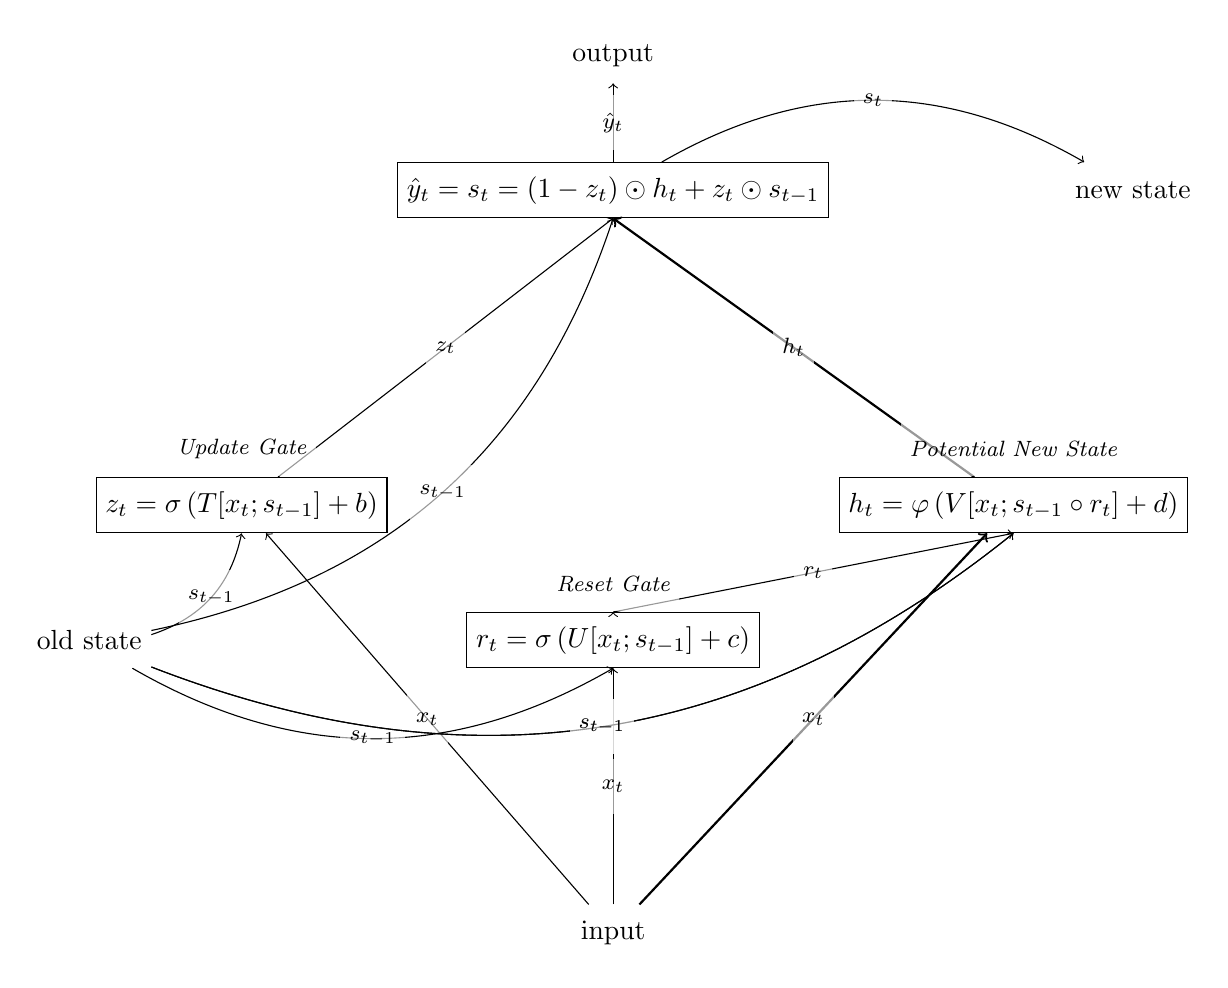
\begin{tikzpicture}[]
		\node(hidden)[layer]{$h_t = \varphi \left( V[x_t; s_{t-1} \circ r_t] + d \right)$};
		\node(reset)[layer, below left=of hidden]{$r_t = \sigma \left( U[x_t; s_{t-1}] + c \right)$};
		\node(update)[layer, above left=of reset]{$z_t = \sigma \left( T[x_t; s_{t-1}] + b \right) $};
		\node(state)[layer, above = 5 of reset]{$\hat{y}_t=s_t = (1-z_t) \odot h_t + z_t \odot s_{t-1}$};
		
		\node(in)[below = 3 of reset]{input};
		\node(stm)[left = 4 of reset]{old state};
		\node(stp)[right = 3 of state]{new state};
		\node(out)[above = of state]{output};
		
		\draw[->] (in) edge node[labe] {$x_t$} (update);	
		\draw[->, bend right] (stm) edge node[labe] {$s_{t-1}$} (update.south);
		\draw[->] (in) edge node[labe] {$x_t$} (reset);	
		\draw[->, bend right] (stm) edge node[labe] {$s_{t-1}$} (reset.south);
		
		\draw[->, thick] (in) edge node[labe] {$x_t$} (hidden);	
		\draw[->, bend right] (stm) edge node[labe] {$s_{t-1}$} (hidden.south);		
		\draw[->] (reset.north) edge node[labe] {$r_t$} (hidden.south);
		\draw[->, bend right] (stm) edge node[labe] {$s_{t-1}$} (hidden.south);
		
		\draw[->, bend right] (stm) edge node[labe] {$s_{t-1}$} (state.south);
		\draw[->, thick] (hidden) edge node[labe] {$h_{t}$} (state.south);
		\draw[->] (update) edge node[labe] {$z_{t}$} (state.south);
		\draw[->, bend left] (state) edge node[labe] {$s_{t}$} (stp);
		\draw[->] (state) edge node[labe] {$\hat{y}_t$} (out);
		
		\node(updatelbl)[labe, above= 0 of update]{Update Gate};
		\node(resetlbl)[labe, above= 0 of reset]{Reset Gate};
		\node(hiddenlbl)[labe, above= 0 of hidden]{Potential New State};
		\end{tikzpicture}
	\end{adjustbox}
\end{figure}



The gated recurrent unit (GRU) is defined by:
\begin{align}
z_t &= \sigma \left( T[x_t; s_{t-1}] + b \right) \\
r_t &= \sigma \left( U[x_t; s_{t-1}] + c \right) \\
%
h_t &= \varphi \left( V[x_t; s_{t-1} \odot r_t] + d \right)  \\
s_t &= (1-z_t) \odot h_t + z_t\odot s_{t-1}\\
\hat{y}_t &= s_t
\end{align}
Where $T$,$U$ and $V$ are the weight-vectors, and $b$,$c$ and $d$ are the bias vectors for the 3 separate layers.

\aside[Trade-off formula]{It may be stating the obvious, 
	but a standard way (and the only sensible way) to trade-off a value between two possible choices: $a$ and $b$,
	when given a preference level for the first as $p$ (a number between zero and one) is $(p)a+(1-p)b$.
	If $p$ is interpreted as the probability of $a$ being the correct value of a random variable, with $b$ as the other possible value, then this is the expected value of that random variable.}

This may look complex, but it can be broken down into parts.
First we can see that like in the basic RU, the output and the state are the same value.

$h_t$ is our core layer, as in the basic cell.
However, unlike in the basic cell, it does not immediately become the state: $s_t$.
There is a trade-off between the state keeping its old value $s_{t-1}$, and getting the hidden layer value $h_t$.
This trade-off is element-wise controlled by $z_t$ which is valued between 0 and 1 (due to the sigmoid unit).
When an element of $z_t$ is $1$, then the value of $s_{t-1}$ for the corresponding element is kept.
Conversely, when the $z_t$ element is $0$,  then the element of the new state is fully given by $h_t$.

$z_t$ is often called the \emph{update gate} as it controls (``gates'') how much the state is updated using the new value in $h_t$.
The update-gate sub-network uses the previous state $s_{t-1}$ and present input $x_t$ to make this determination.

\aside[Multiplication, Concatenation, and Addition]{
	It is important to grasp that the product of a matrix and the concentration of two vectors can also be expressed as the sum of the product of a block of that matrix 
	The area the same thing.
	
	$W\cdot [a; b] = U\cdot a + V\cdot b$  
	if  $W=[U\; V]$
	
	For $[a;b]$ being the vertical concatenation of the vectors (considered as column matrices) 
	and  $[U\; V]$ the horizontal concatenation of the  matrices respectively.
	
	The difference is purely notation.
}

The \emph{reset gate} is loosely similar.
$r_t$ controls how much influence the past state $s_{t-1}$ has on calculating the new value of $h_t$ -- which is the new potential state/output as discussed.
It is perhaps clearer if $h_t$ is reformulated to split $V$ into the terms that multiply with $x_t$ and the terms that multiply with $s_{t-1}$:
%
\begin{align}
h_t &= \varphi \left( \sigma \left( V[x_t; s_{t-1} \odot r_t] + d \right) \right) \\
&= \varphi \left( \sigma \left( V_x x_t + V_s r_t \odot s_{t-1} + d \right) \right)
\end{align}
%
It $r_t$ is called the reset-gate because it wipes the effect of the old-state in calculating the potential new state $h_t$.
When $r_t$ is reduced to zero, then the updated value for $h_t$ is as if $s_{t-1}$ was just like for the initial zero-vector state -- it is zeroed out by $r_t$.
If the update gate $z_t$ is high then it would fully reset the system.


Notice that when $z_t=0$ and $r_t=1$ then the system is identical to the Basic RU.
This could be achieved by setting suitably large biasses.
However, the system is more flexible than that, 
since $z_t$ and $r_t$ are themselves very similar to Basic RUs -- though they do not control their own state.
The gates can behaver differently based on the inputs and states to recognise important information that must be stored.



\subsection{LSTM Recurrent Unit}\label{sec:ltsm}
The LSTM is most well known RNN unit, the term is very nearly interchangeable with RNN today.
The original form was proposed by \tcite{hochreiter1997long}.
The form in current use is a variant from \tcite{gers1999learning}.

LSTM uses a compound state, comprised of the units previous output, and an addition state vector called the cell.
we write $s_t = (c_t, \hat{y}_t)$,
to fit the normal formulation,
though for maths it is easier to work with these in parts.

\aside[Biasing the Forget Gate]{
	Practically, it is important to initially set the forget gate bias to 1.
	Unlike all the other initialisation in the networks to 0 (or a small random number eg \texttt{randn(0.01)}).
	Equvielently one can also just add a constant additional bias term of ${+}1$ to the forget gate equations.
	This has been show to benefit almost all used of LSTM \parencite{gers1999learning,jozefowicz2015empirical}.
	This is the default in most frameworks (though only recently patched in some).
}

\begin{align}
s_t &= (c_t, \hat{y}_t)\\
%
i_t &= \sigma \left( W[x_t; \hat{y}_{t-1}] + d \right) \\
f_t &= \sigma \left( T[x_t; \hat{y}_{t-1}] + b \right) \\
o_t &= \sigma \left( U[x_t; \hat{y}_{t-1}] + k \right) \\
%
h_t &= \tanh \left( V[x_t; \hat{y}_{t-1}] + a \right) \\
c_t &=  i_t\odot h_{t} + f_t \odot c_{t-1} \\
\hat{y}_t &= o_t \odot \varphi(c_t)
\end{align}



In LSTM there are 3 gate sub-networks:
the input gate $i_t$, the forget gate $f_t$, and the output gate $o_t$.

Together the input and forget-gates take the purpose of the GRU's update-gate.
Consider the case if $o_t=1$ and $\varphi$ is the identify function,
and with $i_t=1-f_t$, that would make the value for $c_t$ very similar to GRU's $s_t$ (and $\hat{y}_t$ identical)
\pdfcomment{Should I rewrite out the equation in this form, or would that be more confusing?}

Individually, the forget gate $f_t$ controls the extent that previous value of the cell is used,
and the input gate $i_t$ controls the extent to which the new potential value $h_t$ is used for the new value of $c_t$.

The output-gates obvious purpose is to gate the output $y_t$.
However, as the output forms part of the state,
this has an effect on the networks next time step.
Loosely this can be seen as similar to the GRU's reset gate.
If we substitute the value for $\hat{y}_{t-1} = o_{t-1}\cdot\varphi(\odot c_{t-1})$
into $h_t$:
\begin{align}
h_t &= \tanh \left( V[x_t; \hat{y}_{t-1}] + a \right) \\
&=\tanh \left( V[x_t; o_{t-1}\cdot\varphi(\odot c_{t-1})] + a \right)
\end{align}
Similar for $o_t$, $f_t$ and $o_t$ as for $h_t$.
It can be seen that at the previous time step setting an element of $o_{t-1}$ to zero effectively removes the effect of the previous cell-state from the equations for all the gates and the the potential new cell $h_t$.
Thus resetting the network.


\begin{figure}
	\caption{A LSTM Recurrent unit. It may seem complex, and that is basically because it is. However, it can be broken down into understandable parts.}
	\label{fig:lstm}
	\begin{adjustbox}{max width=\textwidth}
		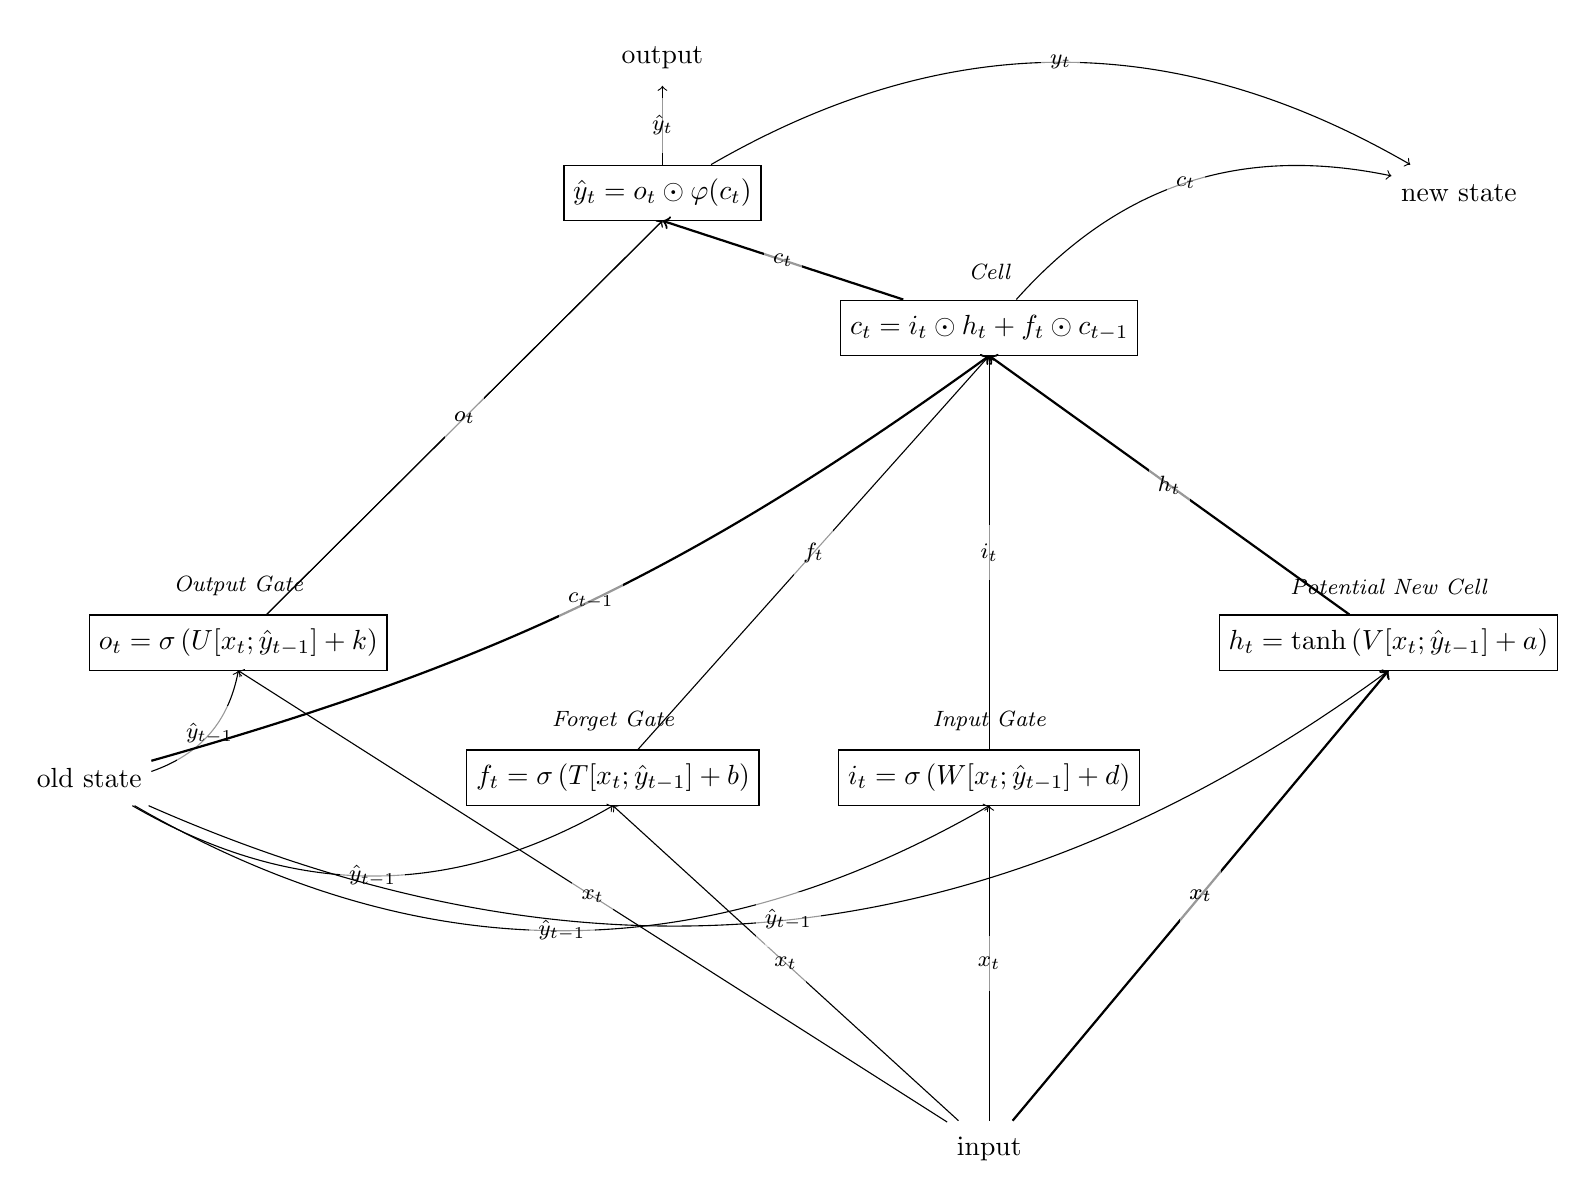
\begin{tikzpicture}[]
		\node(hidden)[layer]{$h_t = \tanh \left( V[x_t; \hat{y}_{t-1}] + a \right) $};
		\node(igate)[layer, below left=of hidden]{$i_t = \sigma \left( W[x_t; \hat{y}_{t-1}] + d \right)$};
		\node(fgate)[layer, left=of igate]{$f_t = \sigma \left( T[x_t; \hat{y}_{t-1}] + b \right)$};
		\node(ogate)[layer, above left=of fgate]{$o_t = \sigma \left( U[x_t; \hat{y}_{t-1}] + k \right)$};
		\node(state)[layer, above = 5 of igate]{$c_t =  i_t\odot h_{t} + f_t \odot c_{t-1}$};
		\node(preout)[layer, above left = of state]{$\hat{y}_t = o_t \odot \varphi(c_t)$};
		
		\node(in)[below = 4 of igate]{input};
		\node(stm)[left = 4 of fgate]{old state};
		\node(stp)[right = 8 of preout]{new state};
		\node(out)[above = of preout]{output};
		
		
		\node(flbl)[labe, above= 0 of fgate]{Forget Gate};
		\node(ilbl)[labe, above= 0 of igate]{Input Gate};
		\node(olbl)[labe, above= 0 of ogate]{Output Gate};
		\node(hiddenlbl)[labe, above= 0 of hidden]{Potential New Cell};
		\node(statelbl)[labe, above= 0 of state]{Cell};
		
		\foreach \gate in {fgate, igate, ogate, hidden}{
			\draw[->, bend right] (stm) edge node[labe] {$\hat{y}_{t-1}$} (\gate.south);
			\draw[->] (in) edge node[labe] {$x_{t}$} (\gate.south);
		};
		\draw[->, bend right=10, thick] (stm) edge node[labe] {$c_{t-1}$} (state.south);
		
		\draw[->, thick] (in) edge node[labe] {$x_{t}$} (hidden.south);
		
		
		\draw[->] (fgate) edge node[labe] {$f_{t}$} (state.south);
		\draw[->] (igate) edge node[labe] {$i_{t}$} (state.south);
		\draw[->, thick] (hidden) edge node[labe] {$h_{t}$} (state.south);
		
		
		
		\draw[->] (ogate) edge node[labe] {$o_{t}$} (preout.south);
		\draw[->] (ogate) edge node[labe] {$o_{t}$} (preout.south);
		
		\draw[->] (preout) edge node[labe] {$\hat{y}_{t}$} (out.south);
		
		\draw[->, thick] (state) edge node[labe] {$c_{t}$} (preout.south);
		
		\draw[->, bend left] (state) edge node[labe] {$c_{t}$} (stp);
		\draw[->, bend left] (preout) edge node[labe] {$y_{t}$} (stp);
		
		
		
		\end{tikzpicture}
	\end{adjustbox}
\end{figure}

\section{Further Variants}
\subsection{Deep Variants}
One can have a deep RNN.
This is done by stacking additional recurrent units above the existing ones.
Attaching, the unit output as the unit input of the layer above.
The result can be interpreted as a single, deep recurrent unit.

\subsection{Bidirectional RNNs}\label{sec:bidirection-rnns}
A Bidirectional RNN is similar to deep variants \pcite{schuster1997bidirectional}.
This is effectively using using two RNNs so that the input can be processed from both temporal directions.
The forward and backwards RNNs both take the same input at each timestep, but are other wise fully distinct.
The unit outputs at each time step are concatenated before passing for further processing.

This is not so useful in most decoder RNNs, the number of outputs (time steps) of a decoder RNN is not known except by running them until an end-marker is output.
However, there are absolutely no issues when using them for an encoder as all the inputs are known in advance as it is processed one full input at a time.
Similar is true for a matched-sequence RNN, when real-time output is not required, and the sequence can be broken up into blocks.


\subsection{Other RNNs}
There also exist many other RNNs.
Some are similar in structure to those discussed and can be analysed similarly via their recurrent units.
Such as the two models of \tcite{mikolovLongerSTM}, which incorporate a decaying sum of past states into the current state (either gated, or constant).
Other networks incorporate various other data-structures (or analogies to such structures) into there recurrent structure:
such as stacks \tcite{stacklstm}, pointers/arrays \tcite{MemoryNN}, or tapes \tcite{DBLP:journals/corr/GravesWD14}.

At natural language is primarily a sequential task, RNNs in various forms will be discussed in almost every chapter of this book.

%\printbibliography

\end{document}